\chapter{The Full Transformer (Encoder-Decoder)}

By now you understand the building blocks: scaled dot-product attention, multi-head attention, feed-forward networks, residual connections, and layer normalization. Chapters~1 and~2 showed how these components form a transformer block. This document steps back to the original architecture from ``Attention Is All You Need'' (Vaswani et al., 2017) and explains how those blocks are arranged into a full encoder-decoder model for machine translation.

We are not building this architecture ourselves --- our BabyGPT will use only the decoder half. But understanding the full picture is necessary to appreciate what GPT keeps, what it drops, and why.

\section{The Sequence-to-Sequence Problem}

Machine translation takes a sentence in one language and produces the equivalent sentence in another. More broadly, many problems have this shape: an input sequence goes in, and a different-length output sequence comes out. Summarization (long document in, short summary out), speech-to-text (audio frames in, words out), and even question answering (context + question in, answer out) are all sequence-to-sequence tasks.

The \textbf{encoder-decoder} paradigm for handling this predates transformers. Sutskever et al.\ (2014) used two RNNs: an encoder RNN reads the input sequence token by token and produces a final hidden state (a single vector), then a decoder RNN generates the output sequence from that vector one token at a time.

The problem is immediate: compressing an arbitrarily long input sentence into a single fixed-size vector is a severe bottleneck. Information is inevitably lost, and the effect gets worse as the input sequence grows. A 50-word sentence and a 5-word sentence both get squeezed into the same-size vector.

Bahdanau et al.\ (2015) solved this by introducing \textbf{attention} into the encoder-decoder RNN. Instead of using only the encoder's final hidden state, the decoder at each time step computes a weighted sum over \textit{all} of the encoder's hidden states. The decoder learns to focus on the relevant parts of the input as it generates each output token. This was the original attention mechanism.

The transformer takes this idea and makes it the entire architecture. There are no recurrent connections at all --- just attention, feed-forward networks, and residual connections. The encoder uses self-attention to build rich representations of the input, the decoder uses self-attention to build representations of the output so far, and cross-attention lets the decoder read from the encoder. The result is a model that is more parallelizable and more powerful than RNN-based approaches.

\section{The Transformer Encoder}

The encoder is a stack of $N = 6$ identical layers. Each encoder layer has two sublayers:

\begin{enumerate}
  \item \textbf{Multi-head self-attention} (bidirectional --- no causal mask)
  \item \textbf{Position-wise feed-forward network}
\end{enumerate}

Both sublayers are wrapped with a residual connection and followed by layer normalization (the original paper uses post-norm: \code{LayerNorm(x + Sublayer(x))}).

The structure of the full encoder:

\begin{verbatim}
Input Tokens -> Embedding + Positional Encoding
    -> [EncoderLayer x N]
    -> Encoder Output (B, T_src, d_model)
\end{verbatim}

$B$ is the batch size (number of sentences processed in parallel), $T_{\text{src}}$ is the length of the source sequence (number of input tokens after padding), and $d_{\text{model}}$ is the embedding dimension --- the width of every hidden representation in the model (512 in the base transformer).

The critical difference from the decoder blocks in Chapter~2: \textbf{there is no causal mask}. Every position can attend to every other position. This is \textbf{bidirectional} attention --- position 5 can look at position 10, and position 10 can look at position 5.

Why bidirectional? The encoder processes the entire input at once. When translating ``The cat sat on the mat'' from English to German, the encoder already has the complete input sentence. There is no reason to hide any positions from each other. The word ``cat'' should be able to use context from ``mat'' at the end of the sentence, and vice versa. Restricting the encoder to only look leftward (as a causal mask does) would throw away useful information for no benefit.

The only masking in the encoder is a \textbf{source mask} (also called a padding mask). When training on batches of sentences, shorter sentences are padded to the length of the longest sentence in the batch. We mask out these padding positions so they do not contribute to attention --- they are not real tokens and should not influence the representation of actual tokens.

The output of the encoder is a tensor of shape \code{(B, T\_src, d\_model)}: a sequence of contextualized representations, one per input position. After passing through 6 layers of bidirectional self-attention, each position's representation encodes information from the entire input sequence. Position 3's output vector is not just about the token at position 3 --- it is a representation of that token in the context of all other tokens.

\section{The Transformer Decoder}

The decoder is also a stack of $N = 6$ identical layers, but each decoder layer has \textbf{three} sublayers (not two):

\begin{enumerate}
  \item \textbf{Masked multi-head self-attention} (with causal mask --- same as our GPT blocks from Chapter~2)
  \item \textbf{Multi-head cross-attention} (queries from the decoder, keys and values from the encoder output)
  \item \textbf{Position-wise feed-forward network}
\end{enumerate}

All three sublayers have residual connections and layer normalization.

The decoder generates output tokens one at a time during inference. When translating to German, it generates ``Die'', then ``Katze'', then ``sa\ss{}'', and so on. The causal mask in the first sublayer ensures that when generating token at position $t$, the decoder can only attend to positions 0 through $t$ (no peeking at future tokens it has not generated yet). During training, \textbf{teacher forcing} feeds the correct target sequence shifted by one position, but the causal mask still prevents the model from cheating by looking ahead.

The structure of the full decoder:

\begin{verbatim}
Target Tokens -> Embedding + Positional Encoding
    -> [DecoderLayer x N]
    -> Linear -> Softmax -> Output Probabilities
\end{verbatim}

\section{Cross-Attention: How the Decoder Reads the Encoder}

Cross-attention is the mechanism that connects encoder and decoder. It is the reason the decoder can generate output that is conditioned on the input --- without it, the decoder would just be a language model with no knowledge of the source sentence.

Cross-attention uses the exact same multi-head attention mechanism from Chapter~1, but the queries, keys, and values come from different places:

\begin{itemize}
  \item \textbf{Queries (Q):} from the decoder's current state (the output of the masked self-attention sublayer)
  \item \textbf{Keys (K) and Values (V):} from the encoder's final output
\end{itemize}

Concretely, for decoder layer $l$:

\[\text{CrossAttn}(Q, K, V) = \text{softmax}\left(\frac{Q K^T}{\sqrt{d_k}}\right) V\]

where $Q = H_{\text{dec}}^{(l)} W^Q$, $K = H_{\text{enc}} W^K$, $V = H_{\text{enc}} W^V$.

$H_{\text{dec}}^{(l)}$ is the decoder's hidden state after masked self-attention in layer $l$ (shape \code{(B, T\_tgt, d\_model)}), and $H_{\text{enc}}$ is the encoder's final output (shape \code{(B, T\_src, d\_model)}).

What this means: each decoder position computes attention over all encoder positions. The attention weight matrix has shape \code{(B, h, T\_tgt, T\_src)} --- each target position assigns a weight to each source position. The decoder ``asks questions'' via its queries, and the encoder ``answers'' through its keys and values.

Consider translating ``The cat sat on the mat'' to ``Die Katze sa\ss{} auf der Matte.'' When the decoder is generating ``Katze'' (German for ``cat''), the query vector at that position will, through the attention mechanism, produce high attention weights on ``cat'' in the encoder output. The decoder is learning a soft alignment between source and target.

There is \textbf{no causal mask} in cross-attention --- every decoder position can attend to every encoder position. The entire input is known (the encoder has already processed it), so there is nothing to hide. The only mask applied in cross-attention is the source padding mask, same as in the encoder's self-attention.

This cross-attention mechanism is conceptually the same as Bahdanau attention from the RNN seq2seq world: the decoder attends to the full encoder output when generating each token. But here it is multi-headed (8 heads in the original paper) and computed without any recurrence, making it far more parallelizable.

\section{Embeddings}

\textbf{Token embeddings} are a learned lookup table that maps each token ID (an integer) to a dense vector of size $d_{\text{model}}$:

\concepttag
\begin{lstlisting}
embedding = nn.Embedding(vocab_size, d_model)
# Input: (B, T) tensor of integer token IDs
# Output: (B, T, d_model) tensor of embedding vectors
\end{lstlisting}

Each row of the embedding matrix corresponds to one token in the vocabulary. These vectors are initialized randomly and learned during training. After training, tokens with similar meanings will tend to have similar embedding vectors.

The original paper uses a \textbf{shared embedding matrix} for both the encoder and decoder. This makes sense when the source and target languages share a vocabulary (common with subword tokenization schemes like BPE, which construct a joint vocabulary across both languages).

BPE is covered in detail in Chapter~5, Section 1. Sharing means the model uses one set of embedding vectors for, say, the token ``the'' regardless of whether it appears on the source side or the target side.

\tip{%
\textbf{The $\sqrt{d_{\text{model}}}$ scaling.} The paper multiplies embedding vectors by $\sqrt{d_{\text{model}}}$ before adding positional encodings. This is easy to miss but has a concrete reason. \code{nn.Embedding} initializes its weight matrix from a standard normal distribution, which gives vectors with entries roughly distributed as $\mathcal{N}(0, 1)$. The L2 norm of such a $d_{\text{model}}$-dimensional vector is approximately $\sqrt{d_{\text{model}}}$, meaning each component has magnitude roughly 1. But in practice, many implementations (including the paper's) initialize with variance closer to $1/d_{\text{model}}$, which gives per-component magnitudes of roughly $1/\sqrt{d_{\text{model}}}$. Meanwhile, the sinusoidal positional encodings (described next) have components bounded in $[-1, 1]$, so their per-component magnitude is \textasciitilde{}1. Without scaling, the positional encodings would dominate the token embeddings. Multiplying by $\sqrt{d_{\text{model}}}$ brings the embedding magnitudes up to the same scale as the positional encodings, so neither overwhelms the other.
}

\section{Positional Encoding}

Attention is \textbf{permutation-invariant}: if you shuffle the input tokens, the set of output vectors is the same set (just shuffled the same way). Formally, for any permutation $\pi$:

\[\text{Attention}(\{x_1, x_2, x_3\}) = \text{Attention}(\{x_{\pi(1)}, x_{\pi(2)}, x_{\pi(3)}\})\]

Without positional information, ``the cat sat on the mat'' and ``mat the on sat cat the'' would produce identical representations. Word order clearly matters, so we must inject position information.

The original paper uses \textbf{fixed sinusoidal positional encodings}:

\[PE_{(pos, 2i)} = \sin\left(\frac{pos}{10000^{2i/d_{\text{model}}}}\right)\]

\[PE_{(pos, 2i+1)} = \cos\left(\frac{pos}{10000^{2i/d_{\text{model}}}}\right)\]

where $pos$ is the position in the sequence (0, 1, 2, \ldots) and $i$ is the dimension pair index (0, 1, 2, \ldots, $d_{\text{model}}/2 - 1$).

\tip{%
\textbf{Reading the two formulas.} The goal is to build a matrix $PE$ of shape $(T, d_{\text{model}})$ --- same shape as the token embeddings --- so we can add them element-wise. The two formulas fill this matrix column by column: the first formula fills even columns ($0, 2, 4, \ldots$) with $\sin$, the second fills odd columns ($1, 3, 5, \ldots$) with $\cos$. Columns $2i$ and $2i{+}1$ form a pair that share the same frequency but use $\sin$ and $\cos$ respectively --- like the $x$ and $y$ coordinates of a point on a circle. Each pair oscillates at a different frequency controlled by $i$: pair $i{=}0$ oscillates fast, and the last pair oscillates extremely slowly. The result is that each row (position) gets a unique combination of fast and slow oscillations across its $d_{\text{model}}$ dimensions --- a unique positional fingerprint. This is the matrix that gets added: \code{x = token\_embeddings + PE}.
}

Each pair of dimensions $(2i, 2i+1)$ forms a sinusoid at a different frequency:

\begin{itemize}
  \item Dimensions 0 and 1: wavelength $= 2\pi$ (the fastest oscillation --- the encoding changes rapidly across positions)
  \item Last pair of dimensions: wavelength $= 2\pi \times 10000$ (extremely slow --- the encoding barely changes from one position to the next)
\end{itemize}

The heatmap below shows the positional encoding matrix for 50 positions and 64 dimensions. Each row is one position, each column is one dimension, and color maps to value ($-1$ to $+1$). The left columns oscillate rapidly across positions (high frequency); the right columns change very slowly (low frequency). Each row has a unique pattern --- the positional fingerprint.

\begin{center}
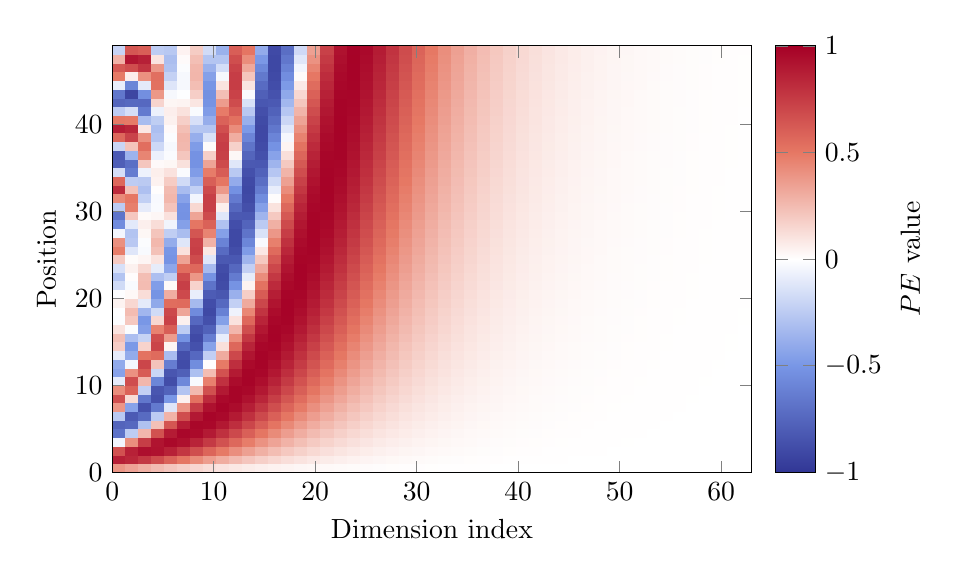
\begin{tikzpicture}
\begin{axis}[
    view={0}{90},
    width=0.8\linewidth,
    height=7cm,
    xlabel={Dimension index},
    ylabel={Position},
    colorbar,
    colorbar style={ylabel={$PE$ value}},
    point meta min=-1,
    point meta max=1,
    samples=50,
    colormap={bluered}{rgb255(0cm)=(49,54,149) rgb255(0.25cm)=(120,150,230)
      rgb255(0.5cm)=(255,255,255) rgb255(0.75cm)=(230,120,100) rgb255(1cm)=(165,0,38)},
]
% sin(pos / 10000^(dim/d_model)) with d_model=64
% 10000^(dim/64) = exp(dim * ln(10000) / 64); ln(10000) = 9.21034
\addplot3[surf, shader=flat, domain=0:63, y domain=0:49]
    {sin(deg(y * exp(-x * 9.21034 / 64)))};
\end{axis}
\end{tikzpicture}
\end{center}

The range of frequencies is geometric, spanning from $2\pi$ to $2\pi \times 10000$. This creates a unique ``fingerprint'' for each position: no two positions have the same pattern of values across all dimensions.

\textbf{The geometric interpretation.} Each dimension pair $(2i, 2i+1)$ can be viewed as a point on a circle rotating at frequency $1/10000^{2i/d_{\text{model}}}$. As position increases, the point traces the circle. The key property is that $PE(pos + k)$ can be expressed as a linear transformation of $PE(pos)$ for any fixed offset $k$:

\[PE(pos + k) = M_k \cdot PE(pos)\]

where $M_k$ is a rotation matrix that depends only on $k$, not on $pos$. This means the model can learn to compute relative positions using linear operations on these encodings.

\textbf{Why sinusoidal and not learned?} The paper argues that sinusoidal encodings may generalize to sequence lengths longer than those seen during training, since the sinusoidal functions are defined for any position. In practice, learned positional embeddings (as used in GPT-1 and GPT-2) work just as well for fixed-length contexts and are simpler to implement. Our BabyGPT in Chapter~4 will use learned positional embeddings.

A PyTorch implementation of sinusoidal positional encoding:

\demotag
{\small\itshape This function is not part of our project --- our GPT uses learned positional embeddings instead. Try it to visualize the encoding patterns.}
\begin{lstlisting}
import torch
import math

def sinusoidal_positional_encoding(max_len: int, d_model: int) -> torch.Tensor:
    """Compute sinusoidal positional encodings.

    Returns:
        (max_len, d_model) tensor of positional encodings.
    """
    pe = torch.zeros(max_len, d_model)
    position = torch.arange(0, max_len, dtype=torch.float).unsqueeze(1)  # (max_len, 1)
    # Compute the denominator in log-space for numerical stability:
    # 10000^(2i/d_model) = exp(2i/d_model * ln(10000))
    div_term = torch.exp(
        torch.arange(0, d_model, 2, dtype=torch.float) * (-math.log(10000.0) / d_model)
    )  # (d_model/2,)

    pe[:, 0::2] = torch.sin(position * div_term)  # even dimensions
    pe[:, 1::2] = torch.cos(position * div_term)  # odd dimensions
    return pe
\end{lstlisting}

The result is added element-wise to the token embeddings: \code{x = token\_embedding * sqrt(d\_model) + positional\_encoding}. These encodings are not learned --- they are computed once and remain fixed throughout training.

\section{The Output Head (Generator)}

After the stack of 6 decoder layers, we need to convert the decoder's output vectors (shape \code{(B, T\_tgt, d\_model)}) into a probability distribution over the vocabulary. This happens in two steps:

\begin{enumerate}
  \item A \textbf{linear layer} projects from $d_{\text{model}}$ to \code{vocab\_size}: the output is a vector of raw scores (logits) for each token in the vocabulary.
  \item \textbf{Softmax} converts these logits into a probability distribution.
\end{enumerate}

\concepttag
\begin{lstlisting}
# After decoder stack:
logits = linear(decoder_output)  # (B, T_tgt, vocab_size)
probs = softmax(logits, dim=-1)  # (B, T_tgt, vocab_size)
\end{lstlisting}

\textbf{Weight tying.} The original paper shares the weight matrix between the token embedding layer and this output projection layer. The embedding matrix has shape \code{(vocab\_size, d\_model)}. The output linear layer needs a weight matrix of shape \code{(d\_model, vocab\_size)} --- which is exactly the transpose of the embedding matrix.

Why does this work? Consider what each does: the embedding layer maps a token ID to a vector in $d_{\text{model}}$-dimensional space. The output layer maps a $d_{\text{model}}$-dimensional vector to a score for each token in the vocabulary. When we use the transposed embedding matrix for the output projection, the score for a given token is the dot product between the decoder's output vector and that token's embedding vector. Tokens whose embeddings are similar to the decoder's output get high scores. This is a natural and consistent choice: the model's notion of ``what a token means'' (the embedding) is the same representation it uses to predict the next token.

Weight tying also has a practical benefit: for large vocabularies (32K or more tokens), the embedding matrix is a significant fraction of the model's total parameters. Sharing it with the output layer saves that entire parameter count.

\section{Putting It All Together}

The complete architecture, following the layout from ``Attention Is All You Need'' Figure~1:

\begin{center}
\begin{tikzpicture}[
    box/.style={draw, rounded corners=2pt, minimum width=2.6cm, minimum height=0.55cm,
                align=center, font=\scriptsize\sffamily},
    attn/.style={box, fill=orange!30},
    norm/.style={box, fill=yellow!25},
    ffn/.style={box, fill=blue!15},
    emb/.style={box, fill=orange!20},
    head/.style={box, fill=blue!15},
    lbl/.style={font=\scriptsize\sffamily},
    arr/.style={->, >=stealth, thick},
    res/.style={->, >=stealth, thin, gray},
    every node/.style={inner sep=3pt},
]

% ---- Encoder (left) ----
\def\ex{-2.2}  % encoder x centre

% Input label
\node[lbl] (einput) at (\ex, 0) {Inputs};

% Input Embedding
\node[emb] (eemb) at (\ex, 0.8) {Input Embedding};
\draw[arr] (einput) -- (eemb);

% Positional encoding
\node[lbl] (epe) at (\ex, 1.55) {$\oplus$ Positional Encoding};
\draw[arr] (eemb) -- (epe);

% Encoder N× block
\begin{scope}[on background layer]
  \draw[rounded corners=5pt, fill=gray!12, draw=gray!50]
    (\ex-1.65, 2.0) rectangle (\ex+1.65, 5.0);
\end{scope}
\node[lbl, gray] at (\ex+1.35, 2.2) {$\times N$};

% Encoder sublayers
\node[attn] (esa) at (\ex, 2.7) {Multi-Head Attention};
\draw[arr] (epe) -- (esa);

\node[norm] (en1) at (\ex, 3.35) {Add \& Norm};
\draw[arr] (esa) -- (en1);
% residual
\draw[res] ([xshift=-1.5cm]esa.south) |- (en1.west);

\node[ffn]  (eff) at (\ex, 4.0) {Feed Forward};
\draw[arr] (en1) -- (eff);

\node[norm] (en2) at (\ex, 4.65) {Add \& Norm};
\draw[arr] (eff) -- (en2);
% residual
\draw[res] ([xshift=-1.5cm]eff.south) |- (en2.west);

% ---- Decoder (right) ----
\def\dx{2.2}  % decoder x centre

% Output label
\node[lbl] (dinput) at (\dx, 0) {Outputs (shifted right)};

% Output Embedding
\node[emb] (demb) at (\dx, 0.8) {Output Embedding};
\draw[arr] (dinput) -- (demb);

% Positional encoding
\node[lbl] (dpe) at (\dx, 1.55) {$\oplus$ Positional Encoding};
\draw[arr] (demb) -- (dpe);

% Decoder N× block
\begin{scope}[on background layer]
  \draw[rounded corners=5pt, fill=gray!12, draw=gray!50]
    (\dx-1.65, 2.0) rectangle (\dx+1.65, 6.65);
\end{scope}
\node[lbl, gray] at (\dx+1.35, 2.2) {$\times N$};

% Decoder sublayers
\node[attn] (dma) at (\dx, 2.7) {\shortstack{Masked\\[-1pt]Multi-Head Attention}};
\draw[arr] (dpe) -- (dma);

\node[norm] (dn1) at (\dx, 3.45) {Add \& Norm};
\draw[arr] (dma) -- (dn1);
\draw[res] ([xshift=1.5cm]dma.south) |- (dn1.east);

\node[attn] (dca) at (\dx, 4.15) {Multi-Head Attention};
\draw[arr] (dn1) -- (dca);

\node[norm] (dn2) at (\dx, 4.8) {Add \& Norm};
\draw[arr] (dca) -- (dn2);
\draw[res] ([xshift=1.5cm]dca.south) |- (dn2.east);

\node[ffn]  (dff) at (\dx, 5.45) {Feed Forward};
\draw[arr] (dn2) -- (dff);

\node[norm] (dn3) at (\dx, 6.1) {Add \& Norm};
\draw[arr] (dff) -- (dn3);
\draw[res] ([xshift=1.5cm]dff.south) |- (dn3.east);

% ---- Cross-attention arrow (encoder -> decoder) ----
\draw[arr] (en2.east) -- ++(0.3,0) |- (dca.west)
    node[lbl, pos=0.25, above] {K, V};

% ---- Output head ----
\node[head] (lin) at (\dx, 7.2) {Linear};
\draw[arr] (dn3) -- (lin);

\node[head] (soft) at (\dx, 7.85) {Softmax};
\draw[arr] (lin) -- (soft);

\node[lbl] (oprob) at (\dx, 8.5) {Output Probabilities};
\draw[arr] (soft) -- (oprob);

\end{tikzpicture}
\end{center}

Each \code{EncoderLayer} ($\times N$ on the left) contains:
\begin{itemize}
  \item Multi-head self-attention (bidirectional) + residual + LayerNorm
  \item Feed-forward network + residual + LayerNorm
\end{itemize}

Each \code{DecoderLayer} ($\times N$ on the right) contains:
\begin{itemize}
  \item Masked multi-head self-attention (causal) + residual + LayerNorm
  \item Multi-head cross-attention (Q from decoder, K/V from encoder) + residual + LayerNorm
  \item Feed-forward network + residual + LayerNorm
\end{itemize}

\textbf{The original paper's hyperparameters:}

\begin{center}
\begin{tabular}{lll}
\toprule
Parameter & Base Model & Big Model \\
\midrule
Layers ($N$) & 6 & 6 \\
$d_{\text{model}}$ & 512 & 1024 \\
$d_{\text{ff}}$ (FFN hidden dim) & 2048 & 4096 \\
Attention heads ($h$) & 8 & 16 \\
$d_k = d_v$ (per-head dim) & 64 & 64 \\
Total parameters & \textasciitilde{}65M & \textasciitilde{}213M \\
\bottomrule
\end{tabular}
\end{center}

\textbf{Training details:}

\begin{itemize}
  \item \textbf{Hardware:} 8 NVIDIA P100 GPUs
  \item \textbf{Training time:} \textasciitilde{}12 hours for the base model, \textasciitilde{}3.5 days for the big model, on 8 P100 GPUs
  \item \textbf{Optimizer:} Adam ($\beta_1 = 0.9$, $\beta_2 = 0.98$, $\epsilon = 10^{-9}$) with a custom learning rate schedule:
\end{itemize}

\[lr = d_{\text{model}}^{-0.5} \cdot \min(step^{-0.5}, \ step \cdot warmup\_steps^{-1.5})\]

This schedule linearly increases the learning rate for the first \code{warmup\_steps} (4000 steps), then decreases it proportionally to $1/\sqrt{step}$. The warmup prevents large, destabilizing updates early in training when the model's parameters are still random.

\begin{itemize}
  \item \textbf{Regularization:} dropout of 0.1 applied to sublayer outputs, attention weights, and embeddings. Label smoothing of 0.1 (instead of training on hard 0/1 targets, the model trains on targets where the correct class gets probability 0.9 and the remaining 0.1 is spread across all other classes --- this hurts perplexity slightly but improves BLEU score and generalization).
\end{itemize}

\textbf{Results:} On the WMT 2014 English-to-German translation benchmark, the base model achieved 27.3 BLEU and the big model achieved 28.4 BLEU --- state of the art at the time, surpassing all previous models including ensembles.

\section{Looking Ahead}

The encoder-decoder architecture is well-suited for sequence-to-sequence tasks where the input and output are distinct sequences (translation, summarization). But for \textbf{language modeling} --- the task of predicting the next token given preceding tokens --- the encoder and cross-attention are unnecessary overhead. There is no separate ``input'' to encode; the model just reads text and predicts what comes next.

GPT (Radford et al., 2018) simplifies the transformer by keeping only the decoder (with its causal mask), removing the encoder and cross-attention entirely. What remains is a stack of transformer blocks, each containing masked self-attention and a feed-forward network --- exactly the blocks we built in Chapter~2.

Chapter~4 makes this simplification explicit and assembles our BabyGPT.
